%!TEX root=../document.tex
\section{Architektur - A09 Server-Client-Chat}
	\subsection{Aufgabenstellung}
	Verwende das Decorator Pattern, um die Socket-Kommunikation zwischen einem einfachen Server und einem simplen Client (Konsole genügt) zu dekorieren! Die Plaintext-Kommunikation kann z.B. mit einer RSA- oder AES-Verschlüsselung, einer BASE64-Codierung, einem Hashwert / Fingerprint dekoriert werden.
	
	Zeige im Code, dass die unterschiedlichen Dekorierer miteinander kombiniert werden können!
	
	\subsection{Umsetzung}
	Für die Umsetzung wurde wie vorausgesetzt ein Decorator Pattern verwendet.
	Hierbei wird ein angepasster Stream dekoriert. Dieser wird mit einem Socket ausgestattet und dekoriert somit immer die \texttt{write} bzw. die \texttt{read} Methode.
	
	Somit kann bsp. ein \texttt{AESDecorator} erstellt werden, welcher in der \texttt{write} Methode mithilfe eines \textit{Block - Ciphers} den Text verschlüsselt und anschließend in der zugehörigen \textit{read} Methode wieder entschlüsselt.
	
		\subsubsection{UML - Klassendiagramm}
		Das Decorator Pattern wurde nach folgender Struktur umgesetzt.
		\vspace{0.2cm}
		\begin{figure}[!h]
			\begin{center}
				\includegraphics[width=0.76\linewidth]{images/decdiagram.png}
			\end{center}
		\end{figure}
		
			\paragraph{\textit{ChatStream} - Komponente}\mbox{}
			\vspace{0.15cm}\\
			Zu dekorierende Komponente.\\
			Hier wird eine abstrakte Komponente als dekorierende Klasse verwendet, da ein spezielles Interface implementiert werden muss. Die Komponente bietet zwei abstrakte Methoden welche dekoriert werden.
			\begin{itemize}
				\item \textbf{\texttt{public Object read()}}\\
				Daten von dem \textit{ObjectInputStream} lesen und dementsprechend an den Aufrufer zurückliefern. 
				
				\item \textbf{\texttt{public void write(Object o)}}\\
				Ein bestimmtes Objekt mithilfe des \textit{ObjectOutputStream} schreiben.
			\end{itemize}
			
			\paragraph{\textit{CoreChatStream} - Konkrete Komponente}\mbox{}
			\vspace{0.15cm}\\
			Konkrete Implementierung des \textit{ChatStreams} / Komponente.\\
			Diese Klasse extended von der zu dekorierenden Komponente und muss aufgrund der abstrakten Methoden diese auch überschreiben und mit Funktionalität füllen.
			Wie der Name schon beschreibt ist dies die nötigste Grundfunktionalität. In diesem Fall wird ausschließlich ein \textit{Object} gelesen bzw. mit \texttt{read} geschrieben.
			
			\begin{lstlisting}[style=JavaG, caption={Konstruktor and in / out Stream CoreChatStream}]
private ObjectOutput out;
private ObjectInput in;

/**
* {@link CoreChatStream} Constructor
*
* @param socket
* @throws IOException
*/
public CoreChatStream(Socket socket) throws IOException {
	this.out = new ObjectOutputStream(socket.getOutputStream());
	this.in = new ObjectInputStream(socket.getInputStream());
}
			\end{lstlisting}
			
			\begin{minipage}{.5\textwidth}
				\begin{lstlisting}[style=JavaL, caption={read - CoreChatStream}]
 /**
 * Read from an InputStream
 *
 * @return @{@link Object} read Object
 * @throws IOException
 */
 @Override
 public Object read() throws IOException {
	 return this.in.readObject();
 }
				\end{lstlisting}
			\end{minipage}%
			\begin{minipage}{.5\textwidth}
				\begin{lstlisting}[style=JavaR, caption={write - CoreChatStream}]
/**
* Write to an OutputStream
*
* @param o @{@link Object} Object to write
* @throws IOException
*/
@Override
public void write(Object o) throws IOException {
	this.out.writeObject(o);
}
				\end{lstlisting}
			\end{minipage}
			
			\paragraph{\textit{StreamDecorator} - Decorator Komponente}\mbox{}
			\vspace{0.15cm}\\
			Diese Klasse erbt ebenfalls von der zu dekorierenden \textit{ChatStream} Klasse.\\
			Zusätzlich wird ein Attribut meist \texttt{inner} gennant, erstellt welches von dem gleichen Type wie der Decorator Komponente ist in diesem Fall \textit{ChatStream}.
			Dieses Attribut ist sozusagen der innere ChatStream. Sobald nun ein ChatStream mittels dem Decorator dekoriert wird kann mit dem Attribute \texttt{inner}, die inneren zu dekorierenden Methoden aufgerufen werden und somit rekursiv nach innen durchzuarbeiten.
			
			\begin{lstlisting}[style=JavaG, caption={Konstruktor and inner StreamDecorator}]
/**
* Inner ChatStream which will be further decorated
*/
private ChatStream inner;

/**
* {@link StreamDecorator} Constructor
* @param inner
*/
public StreamDecorator(ChatStream inner) {
	this.inner = inner;
}
			\end{lstlisting}
			
			\begin{minipage}{.5\textwidth}
				\begin{lstlisting}[style=JavaL, caption={read - StreamDecorator}]
/**
* @see ChatStream
*
* @return
* @throws IOException
*/
@Override
public Object read() throws IOException {
	return this.inner.read();
}
				\end{lstlisting}
			\end{minipage}%
			\begin{minipage}{.5\textwidth}
				\begin{lstlisting}[style=JavaR, caption={write - StreamDecorator}]
/**
* @see ChatStream
*
* @param o @{@link Object} Object to write
* @throws IOException
*/
@Override
public void write(Object o) throws IOException {
	this.inner.write(o);
}
				\end{lstlisting}
			\end{minipage}
			
			Zudem muss, nachdem der ganze ChatStream \textit{AutoClosable} implementiert, eine \texttt{close} Methode existieren, welche alle inneren Streams regelkonform schließt und auf eventuelle Fehler reagiert.
			
			\begin{lstlisting}[style=JavaG, caption={close StreamDecorator}]
/**
* Closes this resource, relinquishing any underlying resources.
* This method is invoked automatically on objects managed by the
* {@code try}-with-resources statement.
*/
@Override
public void close() throws Exception {
	this.inner.close();
}
			\end{lstlisting}
			

\clearpage


			\paragraph{\textit{AES/Base64... - Decorator} - Die Decorator Komponenten}\mbox{}
			\vspace{0.15cm}\\
			Der wichtigste Zweck dieser Klassen ist, die abstrakten Methoden in diesem Fall \texttt{read} \& \texttt{write} zu implementieren und zu ''dekorieren''.\\
			Diese Klassen erben von der DekoratorKomponente \textit{StreamDecorator} und hat somit Zugriff auf den inneren \textit{ChatStream} und somit letztendlich auf den \textit{CoreChatStream}. Somit kann das banale \texttt{read} und \texttt{write} von der \textit{CoreChatStream} Klasse erweitert oder gar komplett geändert werden.\\
			Beispiel eines Dekorators: \textit{Base64Decorator}
			
			\begin{minipage}{.5\textwidth}
				\begin{lstlisting}[style=JavaL, caption={read - Base64Decorator}]
/**
* @return
* @throws IOException
* @throws ClassNotFoundException
* @see ChatStream
*/
@Override
public Object read() throws IOException {
	Message<String> a = (Message) super.read();
	byte[] msg = a.getMessage().getBytes();
	byte[] decBytes = Base64.getDec().decode(msg);
	System.out.print("base64:" + a.getMessage());
	a.setMessage(new String(decBytes));
	return a;
}
				\end{lstlisting}
			\end{minipage}%
			\begin{minipage}{.5\textwidth}
				\begin{lstlisting}[style=JavaR, caption={write - Base64Decorator}]
/**
* @param o @{@link Object} Object to write
* @throws IOException
* @see ChatStream
*/
@Override
public void write(Object o) throws IOException {
	byte[] msg = ((Message) o).getMessage();
	byte[] encMsg = Base64.getEnc().encode(msg);
	//System.out.println("base64 encoded Message: " + new String(encodedMsg));
	Message<String> old = (Message<String>)o;
	old.setMessage(new String(encMsg));
	this.inner.write(old);
}
				\end{lstlisting}
			\end{minipage}
			
			Mithilfe des Attributs \textit{inner} kann nun auf die inneren Methoden zugegriffen werden.\\
			Das ermöglicht nun das \textbf{Decorator Pattern}. Hier wird in den Methoden \texttt{write} \& \texttt{read} ein Base64 end/dec String erzeugt und dementsprechend mit \texttt{inner/super.read} \& \texttt{inner/super.write} auf den \textit{Input/Output - Stream} geschrieben.
			
			
			\paragraph{Aufruf / Erstellen eines Stream-Decorators}\mbox{}
			\vspace{0.15cm}\\
			Hierfür ist vorallem die Reihenfolge wichtig, da ansonsten beim lesen, vor allem beim entschlüsseln und decoding Fehler auftretet können.
			
			\begin{lstlisting}[style=JavaG, caption={erstellen / Aufrufen eines Decorators}]
try (
	ChatStream stream =
		new Base64Decorator(
			new AESDecorator(
				new CoreChatStream(socket),
				skeySpec,
				iv
		)
	)
) {
			\end{lstlisting}
			
			
\clearpage


\section{Design - Patterns Allgemein}
Es gibt bereits hunderte verschiedene Design-Patterns für alle Anwendungsfälle und Programmiersprachen. Allgemein kann man jedoch den Sinn und Zweck sowie die Hintergrundgedanken als auch Vor \& Nachteile anhand dieser Beispiele gut zusammenfassen und erklären. \cite{wiki1}

Prinzipiell werden Design-Patterns verwendet um Programmcode wiederverwendbar und vor allem übersichtlich zu gestalten. Dafür gibt es zahlreiche Vorlagen und Templates. Im Prinzip gibt es zahllose Baupläne für ein passenden Software Design. Die Schwirigkeit hierbei liegt nun das \textbf{richtige} Pattern auszwählen und anzuwenden. \cite{wiki1}

Des Weiteren bieten bereits \textbf{getestete} Design-Patterns ein zuverlässiges Programmierparadigma und somit können Fehler und Gedankenfehler vorgebeugt werden. Bereits bewiesene Patterns werden mit großer Wahrscheinlichkeit auch für den eigenen Anwendungsfall genügen.

	\subsection{Klassifizierung Design-Patterns \cite{wiki1}}
	Prinzipiell können alle Arten von Design-Patterns in 3 Arten unterteilt werden.
	\begin{itemize}
		\item \textbf{Creational Patterns - [Erzeugungsmuster]}\\
		Dienen der Erzeugung von Objekten. Sie entkoppeln die Konstruktion eines Objekts von seiner Repräsentation. Die Objekterzeugung wird gekapselt und ausgelagert, um den Kontext der Objekterzeugung unabhängig von der konkreten Implementierung zu halten, gemäß der Regel: „Programmiere auf die Schnittstelle, nicht auf die Implementierung!“
		
		\item \textbf{Structural Patterns - [Strukturmuster]}\\
		Erleichtern den Entwurf von Software durch vorgefertigte Schablonen für Beziehungen zwischen Klassen. 
		
		\item \textbf{Behavioral Patterns - [Verhaltensmuster]}\\
		Modellieren komplexes Verhalten der Software und erhöhen damit die Flexibilität der Software hinsichtlich ihres Verhaltens.
	\end{itemize}
	
	Zudem kamen später noch weitere Typen für Entwurfsmuster dazu, welche zu keinen der 3 bereits genannten Typen dazu passte. Beispielsweise für Muster für Objekt rationale Abbildungen.
	Diese dienen der Ablage und dem Zugriff von Objekten und deren Beziehungen in einer relationalen Datenbank


\clearpage


	\subsection{Warum werden Deisgn-Patterns verwendet ?}
	Wie bereits angeschnitten sollen Entwurfsmuster uns dabei helfen unser Design flexibler und eleganter zu gestalten, und somit die Software wiederverwendbar machen. Aber warum sollten wir mehr Aufwand bei der Entwicklung treiben, um in der Software die eben
	genannten Eigenschaften zu realisieren?
	
	Im wesentliche verfolgt die Wiederverwendung von Software 3 wichtigen Zielen.
	
	\begin{itemize}
		\item[\Checkmark] \textbf{Reduzierung des Entwicklungsaufwandes}\\
		Da bereits die schwierige Arbeit des tüftelns getan wurde, muss das Design-Pattern lediglich noch angewendet werden.\cite{pdf1}
		
		\item[\Checkmark] \textbf{Erreichung einer Qualitätsverbesserung}\\
		Da diese Patterns sich offenbar schon bewahrt haben kann man auf jeden Fall davon ausgehen, dass diese auch ''optimal'' umgesetzt sind. Zudem kommt, dass man durch diese Muster gezwungen ist, sich nach diesem Bauplan zu halten, welches selbstverständlich auch die insgesamte Qualität erhöhen kann.
		
		\item[\Checkmark] \textbf{Einheitliche Wartbarkeit}\\
		Nachdem die Qualität gegeben ist, ist ebenfalls ein einheitlicher Code gegeben. Dieser ist natürlich, wenn mehrere Entwickler an einem Programm arbeiten, um einiges einfacher zu warten. Auch wenn der Code lang funktionieren soll und deshalb des öfteren erweitert und erneuert werden soll, können dies Design-Patterns erleichtert. \cite{pdf1}
	\end{itemize}
	
	Hierbei ist jedoch zu sagen, dass zuerst ein größerer Aufwand nötig ist um das richtige Design auszuwählen und anzuwenden.
	
	Zuerst sollte man sich im klaren sein welche verschiedenen Arten von Design-Patterns verwendet werden und anschließend verschiedene Muster ausarbeiten und dementsprechend umsetzten.\cite{pdf1}
	
	Es muss nicht immer nur ein Entwurfsmuster verwendet werden. Diese können auch kombiniert werden um sein Ziel zu erreichen und alle Aufgabenstellungen zu erfüllen.\cite{pdf1}
	

\clearpage


	\subsection{Übersicht aktueller Design-Patterns}
	Übersicht aktuell verwendeter Design-Patterns nach ihrer Klassifizierung.
	
		\subsubsection{Creational - Patterns}
		% Please add the following required packages to your document preamble:
		% \usepackage[table,xcdraw]{xcolor}
		% If you use beamer only pass "xcolor=table" option, i.e. \documentclass[xcolor=table]{beamer}
		\def\arraystretch{1.5}
		\begin{table}[!h]
			\centering
			\label{my-label}
		\begin{tabular}{|c|l|}
			\hline
			\rowcolor[HTML]{FFFFFF} 
			{\color[HTML]{000000} \textbf{Name}} & \multicolumn{1}{c|}{\cellcolor[HTML]{FFFFFF}{\color[HTML]{000000} \textbf{Beschreibung}}} \\ \hline
			Abstract Factory & {\color[HTML]{000000} \begin{tabular}[c]{@{}c@{}}Es wird ein Interface zur Verfügung gestellt, um verbundene\\ Objekte zu Erstellen. Ohne Konkrete Klassen zu spezifizieren\end{tabular}} \\ \hline
			Singelton & Es gibt nur eine Instanz dieser Klasse \\ \hline
			Factory Method & \begin{tabular}[c]{@{}c@{}}Mithilfe von dependency Injection kann die subklasse entscheiden\\ wie die methode zu implementieren ist.\end{tabular} \\ \hline
			Multiton & \begin{tabular}[c]{@{}c@{}}Im Gegensatz zu Singelton.\\ Versichern, dass eine Klasse einen globalen Zugriffspunkt für seine\\ Instanzen hat.\end{tabular} \\ \hline
		\end{tabular}
			\caption{Creational Patterns Übersicht \cite{wiki1}}
		\end{table}
		
		\subsubsection{Structural - Patterns}
		% Please add the following required packages to your document preamble:
		% \usepackage[table,xcdraw]{xcolor}
		% If you use beamer only pass "xcolor=table" option, i.e. \documentclass[xcolor=table]{beamer}
		\def\arraystretch{1.5}
		\begin{table}[!h]
			\centering
			\label{my-label}
			\begin{tabular}{|c|l|}
				\hline
				\rowcolor[HTML]{FFFFFF} 
				{\color[HTML]{000000} \textbf{Name}} & \multicolumn{1}{c|}{\cellcolor[HTML]{FFFFFF}{\color[HTML]{000000} \textbf{Beschreibung}}} \\ \hline
				Decorator & \begin{tabular}[c]{@{}c@{}}Dekorieren einer Klasse bzw. von Methoden. \\Dynamisches anpassen von Funktionalität.\end{tabular} \\ \hline
				Composite & \begin{tabular}[c]{@{}c@{}}Objekte in einer Baumstruktur. Partitioning\\ Design-Pattern. Gruppe in gleicher Art behandelt\end{tabular} \\ \hline
				Marker & Leeres Interfaces um Metadaten zuzuweisen \\ \hline
			\end{tabular}
			\caption{Structual Patterns Übersicht \cite{wiki1}}
		\end{table}
	

\clearpage


		\subsubsection{Behavioral patterns}
		% Please add the following required packages to your document preamble:
		% \usepackage[table,xcdraw]{xcolor}
		% If you use beamer only pass "xcolor=table" option, i.e. \documentclass[xcolor=table]{beamer}
		\def\arraystretch{1.5}
		\begin{table}[!h]
			\centering
			\label{my-label}
			\begin{tabular}{|l|c|}
				\hline
				\rowcolor[HTML]{FFFFFF} 
				\multicolumn{1}{|c|}{\cellcolor[HTML]{FFFFFF}{\color[HTML]{000000} \textbf{Name}}} & {\color[HTML]{000000} \textbf{Beschreibung}} \\ \hline
				Command Pattern & \begin{tabular}[c]{@{}c@{}}Verpacken eines Kommandos in einem Objekt.\\ Support of undoable Operations\end{tabular} \\ \hline
				Strategy Pattern & \begin{tabular}[c]{@{}c@{}}Variieren des ALgorithmus, je nach Client.\\ Kapseln jeder Funktionalität und diese untereinander\\ tauschbar gestalten.\end{tabular} \\ \hline
				Visitor Pattern & \begin{tabular}[c]{@{}c@{}}Kapselung von Operationen auf Elemente einer Objekt - \\ Struktur. Neue Operationen ohne Veränderung von\\ betroffenen Elementklassen.\end{tabular} \\ \hline
			\end{tabular}
			\caption{Behavioral patterns Übersicht \cite{wiki1}}
		\end{table}\textbf{}

\clearpage

\section{Das Decorator Pattern}
Das Decorater Pattern ist weit verbreitet und wird selbstverständlich auch von Java verwendet. Dieses
Pattern ermöglicht es, Funktionalität während der Laufzeit hinzuzufügen ohne die bereits bestehende
Funktionalität eines Objketes zu verändern.

	\subsection{Allgemeines Klassendiagramm}
	\begin{figure}[!h]
		\begin{center}
			\includegraphics[width=0.9\linewidth]{images/dec.png}
		\end{center}
	\end{figure}
	
	\subsection{Grundzüge des Designpatterns}
	Das Decorator - Pattern erlaubt uns das Verhalten bzw. die Funktionalität eines Objektes während der
	Laufzeit zu erweitern, ohne Änderungen direkt am Objekt vorzumehnen
	Das Dekorieren/Erweitern kann statisch, sowie in manche Fällen auch dynamisch erfolgen. Um dies zu
	erreichen wird die Basis Klasse als Decorater Klass implementiert. Dies wird erreicht indem wir diese
	Basis Klasse als Decorater Klasse wrapen. Es gibt 3 Implementations:
	
	\begin{itemize}
		\item \textbf{Inheritance}
		\item \textbf{Wrapper}
		\item \textbf{External}
	\end{itemize}
	

\clearpage

	
	\subsubsection{Inheritance \cite{decoratorDebug}}
	Es wird von der \texttt{Decorater Klasse} geerbt. Alle weiteren Funktionen können anschließend in der Kindklasse implementiert werden.
	
	\begin{lstlisting}[style=JavaG, caption=Decorator Pattern Inheritance \cite{decoratorDebug}]
public class DebugButton extends JButton {
	public DebugButton() {
		addActionListener(new ActionListener() {
			System.out.println("debug message");
		});
	}
}
	\end{lstlisting}
	
	Als Beispiel die \texttt{BufferedInputStream.class} Implementation.
	Jede \texttt{read()} Methode kann den buffer nach der nächsten Portion von Bytes fragen. Falls der Buffer leer ist wurde er wahrscheinlich von der \texttt{super.read()} Methode gefüllt.
	
	\paragraph{Vorteile}\mbox{}\\
	\begin{itemize}
		\item Wir können nahezu jeden Decorator implementieren.
	\end{itemize}
	
	
	\subsubsection{Wrapper \cite{decoratorDebug}}
	Die Idee beim wrapping ist, ein dekoriertes Objekt in dem Decorater Pattern zu verpacken. Das Decorator Pattern leitet requests zu dem gewrapptem Objekt und kann die neue Funktionalität anschließend vor / nach dem forwarden ausführen.
	
	Bsp: \textbf{\texttt{BufferedReader.class}}
	
	\texttt{BufferedReader.class} ist ein Wrapper von \texttt{InputStream}.
	Obwohl es die Klasse \texttt{InputStream} extended ist es ein Wrapper.
	Im Konstruktor von \texttt{BufferedReader} wird ein \texttt{InputStram} initialisiert und behält diesen als instance Variable. Aufrufe können anschließend an den \texttt{InputStream} weitergeleitet werden.
	
	Bsp: \textbf{\texttt{DebugButton}}
	
	Wir wollen den JButton erweitern um einen DebugButton zu erhalten.
	Dieser DebugButton hat dieselben Funktionen wie ein noramler JButton, abgesehen davon, dass er bei jedem Druck eine Message "log msg" ausgibt.
	
\clearpage
	
	\begin{lstlisting}[style=JavaG, caption=Decorator - Wrapper \cite{decoratorDebug}]
public class DebugButton extends JButton implements ActionListener {
	private JButton butt = null;
	public DebugButton(JButton butt) {
		this.butt=butt;
		butt.addActionListener(this);
	}
	public void actionPerformed(ActionEvent e) {
	}
}	
	\end{lstlisting}
	
	\subsubsection{External \cite{decoratorDebug}}
	Um die External Implementierung darzustellen, wird wieder das Bsp mit DebugButton hergenommen.
	Zuerst wird eine \texttt{Decorator Class erstellt}.
	
	\begin{lstlisting}[style=JavaG, caption=Decorator External \cite{decoratorDebug}]
public class DebugDecorator implements ActionListener {
	public void decorateDebug(JButton butt) {
		butt.addActonListenr(this);
	}
	public void undecorateDebug(JButton butt) {
		butt.removeActonListenr(this);
	}
	public void actionPerformed(ActionEvent evt) {
		System.out.println("debug message for button" + src);
	}
}
	\end{lstlisting}
	
	Nun können wir den folgenden Code überall anwenden.
	\begin{lstlisting}[style=JavaG, caption=Decorator External Aufruf\cite{decoratorDebug}]
DebugDecorator decor = new DebugDecorator();
JButton myButt = ...
// Add external decorator 
decor.decorateDebug(myButt);
// Remove external decorator
decor.undecorateDebug(myButt);
	\end{lstlisting}
	

\clearpage


	\subsection{Vor \& Nachteile des Decorator Patterns}
		\subsubsection{Vorteile}
		Die Vorteile bestehen darin, dass mehrere Dekorierer hintereinandergeschaltet werden können; die Dekorierer können zur Laufzeit und sogar nach der Instanziierung ausgetauscht werden. Die zu dekorierende Klasse ist nicht unbedingt festgelegt (wohl aber deren Schnittstelle). Zudem können lange und unübersichtliche Vererbungshierarchien vermieden werden.
		
		\subsubsection{Nachteile}
		Das Muster hat eine Gefahr: Da eine dekorierte Komponente nicht identisch mit der Komponente selbst ist (als Objekt), muss man beim Testen auf Objekt-Identität vorsichtig sein. (Ein Vergleich kann falsch ausgehen, obwohl dieselbe Komponente gemeint ist.) Zudem müssen bei der Verwendung von dekorierten Komponenten die Nachrichten vom Dekorierer an das dekorierte Objekt weitergeleitet werden.
	
	\subsection{Anwendungsfälle in der Java API}
	Java verwendet in zahlreichen Packages das Decorator Pattern.
	Das erleichtert dem Entwickler einiges und kann auch einfach umgesetzt werden. Beispielsweise im Package \textit{java.io} oder \textit{java.util.Collection} wird das Decorat-Pattern angewendet.
	
	\subsubsection{Package \textit{java.io}}
	\textbf{Die Struktur des InputStreams ist wie folgt aufgebaut:\cite{javaApi}}
	\vspace{5mm}
	\texttt{
		\\class java.io.InputStream\\
		\hspace*{20mm} class java.io.FileInputStream\\
		\hspace*{40mm} class java.io.BufferedInputStream\\
		\hspace*{40mm} class java.util.zip.CheckedInputStream\\ 
		\hspace*{40mm} class java.io.DataInputStream\\ 
		\hspace*{40mm} class java.security.DigestInputStream\\
		\hspace*{40mm} class java.util.zip.InflaterInputStream\\
		\hspace*{60mm} class java.util.zip.GZIPInputStream\\
		\hspace*{60mm} class java.util.zip.ZipInputStream\\
		\hspace*{40mm} class java.io.LineNumberInputStream\\
		\hspace*{40mm}  class java.io.PushbackInputStream\\
	}
	Um nun beispielsweise eine Datei \texttt{foo.zip} kann von folgendem Stream gelesen werden:
	
	\begin{lstlisting}[style=JavaG, caption=Example Decorator java.io \cite{decoratorDebug}]
	DataInputStream input = new DataInputStream ( new ZipInputStream ( new FileInputStream ("foo.zip") ) );
	\end{lstlisting}
	
	\texttt{class java.io.FileInputStream} ist ebenfalls in der \texttt{class java.io.InputStream} und beinhaltet somit das feld vom Typ \texttt{InputStream} zu dem alle Aufrufe delegeirt werden.
	Einfach gessagt fügt das Decorator Pattern funktonaliät hinzu ohne das Interface zu ändern.
	
	\paragraph{Funktionsweise \cite{decoratorStack} \cite{threePatterns}}\mbox{}\\
	Wenn wir uns InputStream und seine Implementationen genauer ansehen, dann bemerken wir, dass die Implementations wie BufferedInputStream / FilterInputStream im Konstruktor eine Instanz von der abstrakten Klasse. Dies ist eins der Merkmale eines typischen Decorater Patterns. (Dies gilt auch für Konstruktoren, welche eine Instanz von demselben Interface nimmt)
	
	\vspace{1cm}
	
	\begin{figure}[!h]
		\begin{center}
			\includegraphics[width=0.9\linewidth]{images/api-inputstream-gr.png}
			\caption{InputStream - Uml Class Diagram \cite{pdf1}}
			\label{Decorator Pattern - Klassen Diagramm}
		\end{center}
	\end{figure}
		

\clearpage


	\subsection{package \texttt{javax.swing} \cite{pdf1} \cite{javaApi}}
	An zahlreichen Stellen in GUI-Bibliotheken werden GUI-Komponenten dekoriert. Ein typisches Beispiel ist die JScrollPane von Swing.
	
	\begin{figure}[!h]
		\begin{center}
			\includegraphics[width=0.8\linewidth]{images/api-jscrollpane.png}
			\caption{JScrollPane - Uml Class Diagram \cite{pdf1}}
			\label{Decorator Pattern - Klassen Diagramm}
		\end{center}
	\end{figure}
	
	Soll eine JTextArea oder ein JTree Scrollbalken erhalten, so muss man das Objekt nur einer JScrollPane als Konstruktorparameter übergeben und das JScollPane-Objekt stattdessen (es ist ja auch eine Component) auf den Container (JPanel/JFrame) hinzufügen. Soll nun die Component gezeichnet werden, so fügt das JScrollPane-Objekt dem JTextArea-Objekt das nötige Verhalten für Scrollbalken hinzu.
	
	\begin{lstlisting}[style=JavaG, caption=Example Decorator javax.swing.JScrollPane \cite{pdf1}]
	JTextArea textComponent = new JTextArea(12,20); 
	JScrollPane scrollComponent = new JScrollPane(textComponent); 
	add(scrollComponent); 
	//oder add(new JScrollPane(new JTextArea(12,20)); 
	\end{lstlisting}


\clearpage


\section{Das Observer Pattern}
Das Observer Pattern auch Beobachter Pattern basiert auf dem Prinzip vom allbekannten abonnieren.
Man abonniert von einem \textit{Observable} und wird zum \textit{Observer}. Anschließend kann nun je nach Implmentierung nach dem \textbf{\textit{Pull}} oder nach dem \textbf{\textit{Push}} Prinzip ein Datenstream geupdatet werden.

	\subsection{Allgemeines Klassendiagramm}
	\begin{figure}[!h]
		\begin{center}
			\includegraphics[width=0.9\linewidth]{images/obs.png}
		\end{center}
	\end{figure}
	
	\subsection{Grundzüge des Observer Patterns}
	Es gibt immer einen zu abonnierenden Observable und ein Abonneten den Observer. Hierbei ist es üblich, dass man einen neuen Subsriber mit der \texttt{register} Methode hinzufügen kann. Um dies zu gewährleisten werden alle Subscriber anschließend in einer Art Liste verwaltet und somit in der \texttt{register} Methode dieser Liste hinzugefügt.
	
	Ebenfalls soll es möglich sein sich zu trennen und unsubscriben. Dies wird mit der Methode \texttt{unregister} gewährleistet. Desweiteren ist nun noch abhängig ob nach dem Pull oder Push Prinzip gearbeitet wird. Wird ein Push Prinzip verwendet, so hat meist der Observer eine \texttt{update} Methode und sobald das Observable \textbf{notified} wird, so wird mittels einer Schleife alle Observer in der Liste iteriert und geupdatet.
		

\clearpage


	\subsubsection{Beispiel: Messstation / Wetterstation \cite{new}}
	er Entwurf soll es ermöglichen verschiedene Anzeigen zur Darstellung der Wetterdaten einzubinden, ohne grössere Änderungen am bestehenden Code durchzuführen.
	
	Deshalb soll auf eine Schnittstelle anstatt auf eine Implementierung gearbeitet werden.
	Die Wetterstation ist das \textbf{Subjekt}, welches von den Anzeigen als \textbf{Beobachter} beobachtet wird und die bei einer Änderung der Daten benachrichtigt werden. 
	
	Das Subjekt benötigt daher Methoden, die es ermöglichen Beobachter an- und abzumelden sowie über Änderungen zu benachrichtigen. Die Beobachter selbst benötigen eine Methode, die bei einer Änderung vom Subjekt aufgerufen wird und die Änderung mitteilt. Da in dem Beispiel auch eine Anzeige für die Wetterdaten verwendet wird, wird dafür ebenfalls eine Schnittstelle definiert, die die Anzeige aktualisiert.
	
	\paragraph{Klassendiagramm \cite{new}}\mbox{}\\
	\begin{figure}[!h]
		\begin{center}
			\includegraphics[width=0.9\linewidth]{images/obs1.png}
		\end{center}
	\end{figure}


\clearpage


	\paragraph{Akteuere \cite{new}}\mbox{}
	\vspace{0.1cm}
	\begin{itemize}
		\item \textbf{Subject (Subjekt)}\\
		Definiert eine Schnittstelle für die An- und Abmeldung von Beobachtern sowie zur Benachrichtigung der Beobachter über Zustandsänderungen.
		
		\item \textbf{ConcreteSubject (KonkretesSubjekt)}\\
		Implementiert die Schnittstelle des Subjekts. Speichert den Zustand des Objekts und benachrichtigt alle Beobachter über Zustandsänderungen.
		
		\item \textbf{Observer (Beobachter)}\\
		Definiert eine Schnittstelle zur Benachrichtigung über die Zustandsänderung des Subjekts.
		
		\item \textbf{ConcreteObserver (KonkreterBeobachter)}\\
		Implementiert die Schnittstelle zur Benachrichtigung über die Zustandsänderung eines konkreten Subjekts.
	\end{itemize}
	
	\subsection{Vor \& Nachteile des Observer Patterns}
		\subsubsection{Vorteile \cite{wikiobs}}
		Observer und Observables können unabhängig voneinander variiert werden. Diese sind ebenfalls voneinander lose gekoppelt und die Verbindung kann jederzeit getrennt werden.
		
		Das beobachtete Objekt braucht keine Kenntnis über die Struktur seiner Beobachter zu besitzen, sondern kennt diese nur über die Beobachter-Schnittstelle. Ein abhängiges Objekt erhält die Änderungen automatisch. Es werden auch Multicasts unterstützt.
		
		\subsubsection{Nachteile \cite{wikiobs}}
		Änderungen am Subjekt führen bei großer Beobachteranzahl zu hohen Änderungskosten. Außerdem informiert das Subjekt jeden Beobachter, auch wenn dieser die Änderungsinformation nicht benötigt. Zusätzlich können die Änderungen weitere Änderungen nach sich ziehen und so einen unerwartet hohen Aufwand haben.
		
		Der Mechanismus liefert keine Information darüber, was sich geändert hat. Die daraus resultierende Unabhängigkeit der Komponenten kann sich allerdings auch als Vorteil herausstellen.
	
\clearpage

	
	\subsection{Anwendungsfälle des Observer / Beobachter Patterns}
	Das klassische Anwendungsbeispiel in der Java-API ist das Eventhandling von AWT/Swing. Die GUI-Komponenten sind dabei die Subjects, bei den sich Listener, die Observer, registrieren können. Findet eine Userinteraktion auf der Komponente statt, so werden alle registrierten Listener benachrichtigt.
	
	Der Aufbau wird im folgendem am Beispiel von Buttons und dem dazugehörigen Action- und ChangeListenern dargestellt.
	
	\paragraph{Klassendiagramm \cite{obss}}\mbox{}\\
	\begin{figure}[!h]
		\begin{center}
			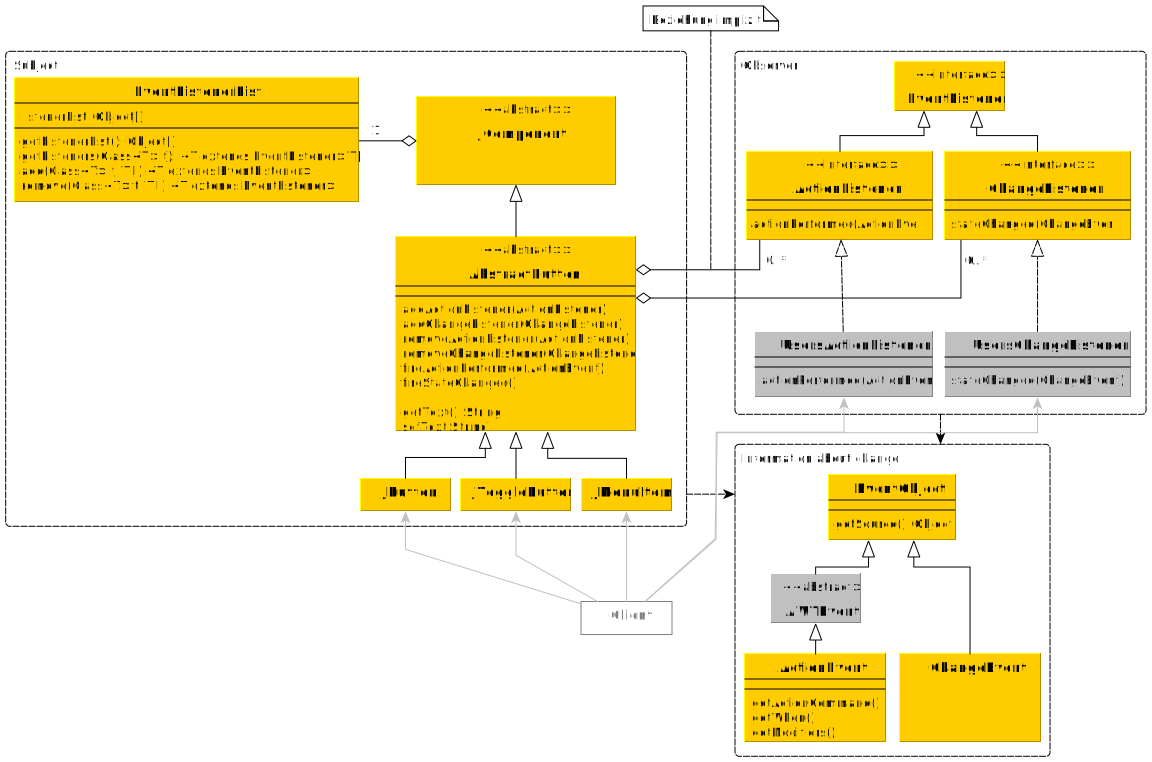
\includegraphics[width=0.9\linewidth]{images/api-eventhandling.png}
		\end{center}
	\end{figure}
	
	Jeder Swing-Button erbt von AbstractButton Methoden zum An- und Abmelden von Listenern, sowie eine Methode fireActionPerformed() (bzw. fireStateChanged()) zur Benachrichtigung der entsprechenden Listener. Diese müssen die Aktualisierungsmethode actionPerformed(ActionEvent) bzw. stateChanged(ChangeEvent)) implementieren.
\clearpage